\documentclass{beamer}

\usepackage[utf8]{inputenc}
\usepackage{graphicx}

\title{Stay Safe in a Pandemic}
\subtitle{tips for those cloistered}
\author{Eric Herman}
%\institute{MariaDB Foundation}
\date{2021-02-06}

\begin{document}

\frame{\titlepage}

\begin{frame}
\frametitle{Order a Brew Kit}
\begin{figure}
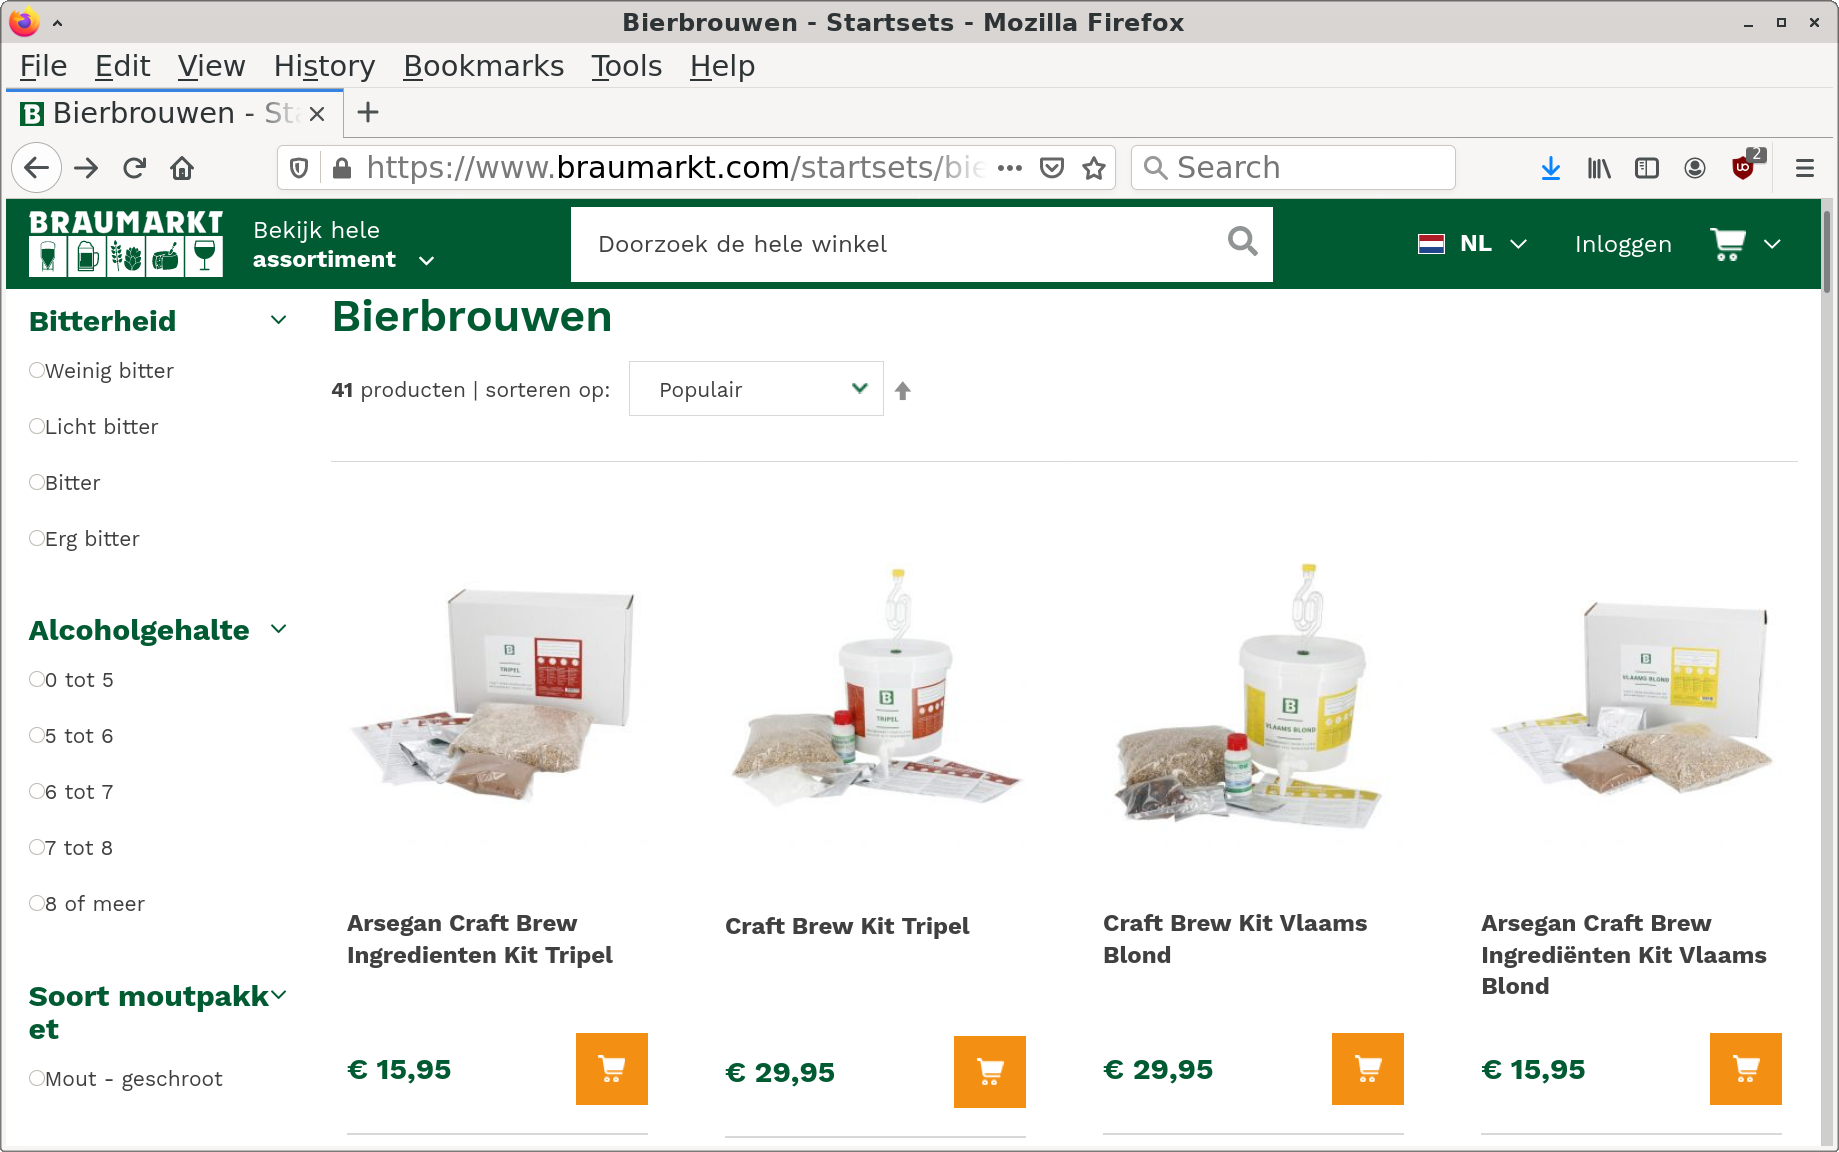
\includegraphics[width=\linewidth]{images/get-a-brew-kit.png}
\end{figure}
\end{frame}

\begin{frame}
\frametitle{Make the wort}
Which is how our cat got his name:
\begin{figure}
\includegraphics[height=.7\textheight]{images/wort-gets-hist-name.jpeg}
\end{figure}
\end{frame}

\begin{frame}
\frametitle{Wait for it to ferment}
In about two weeks, you will be able to bottle:
\begin{figure}
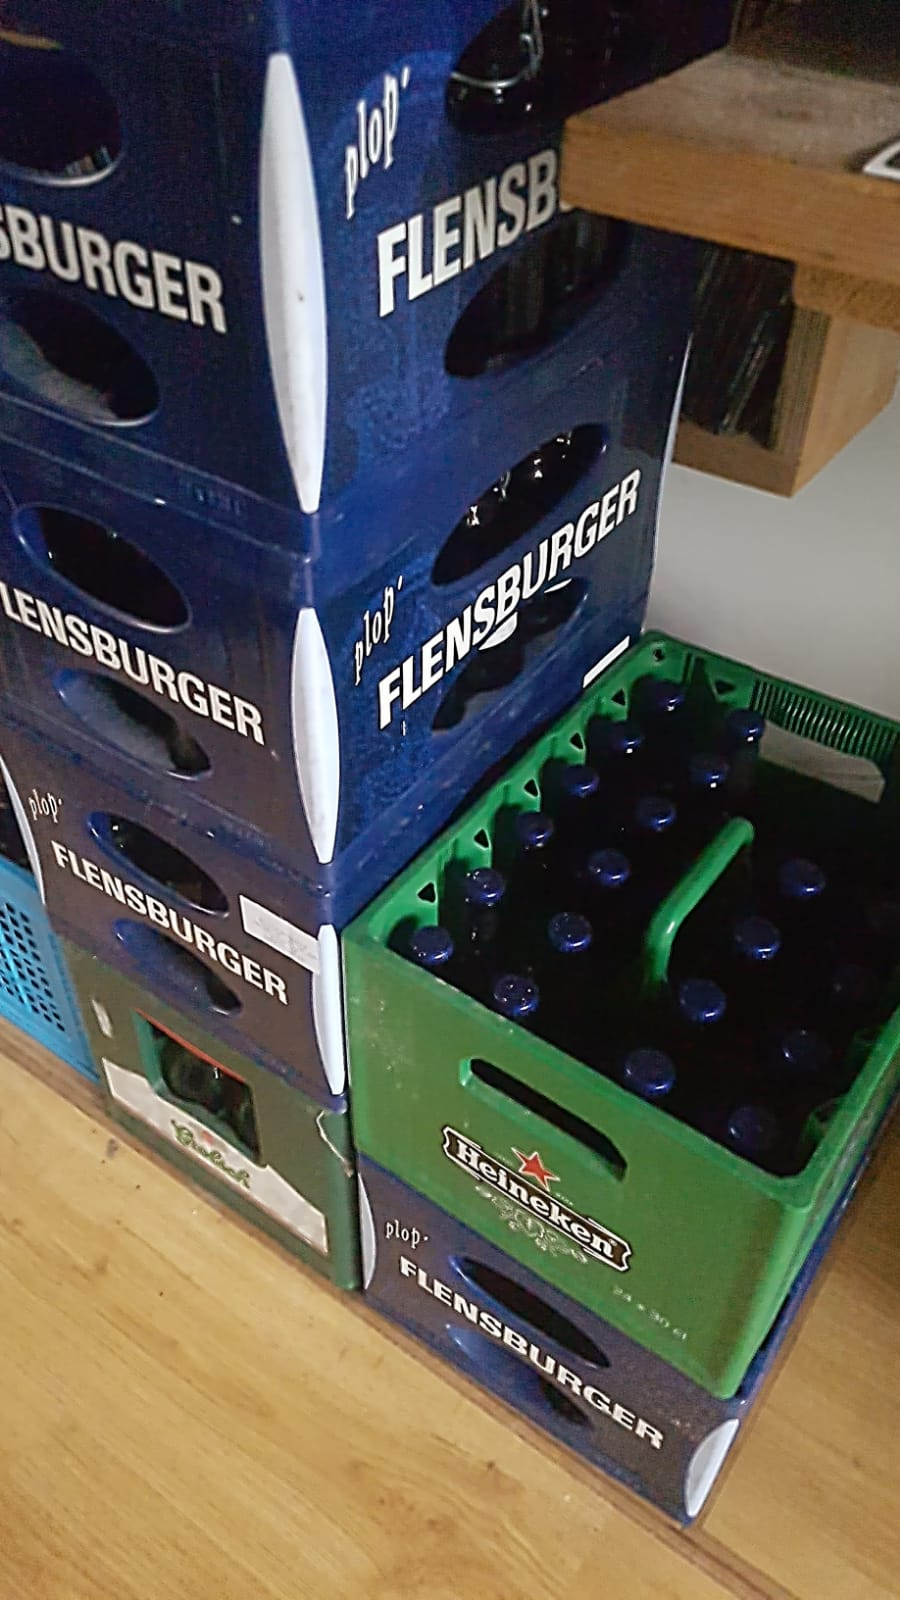
\includegraphics[height=.7\textheight]{images/make-a-batch.jpeg}
\end{figure}
But you need to wait a month or more if you wish to drink it
\end{frame}

\begin{frame}
\frametitle{But we have other plans}
\huge{We want to keep ourselves extra safe!}
\end{frame}

\begin{frame}
\frametitle{Order a decorative still}
\begin{figure}
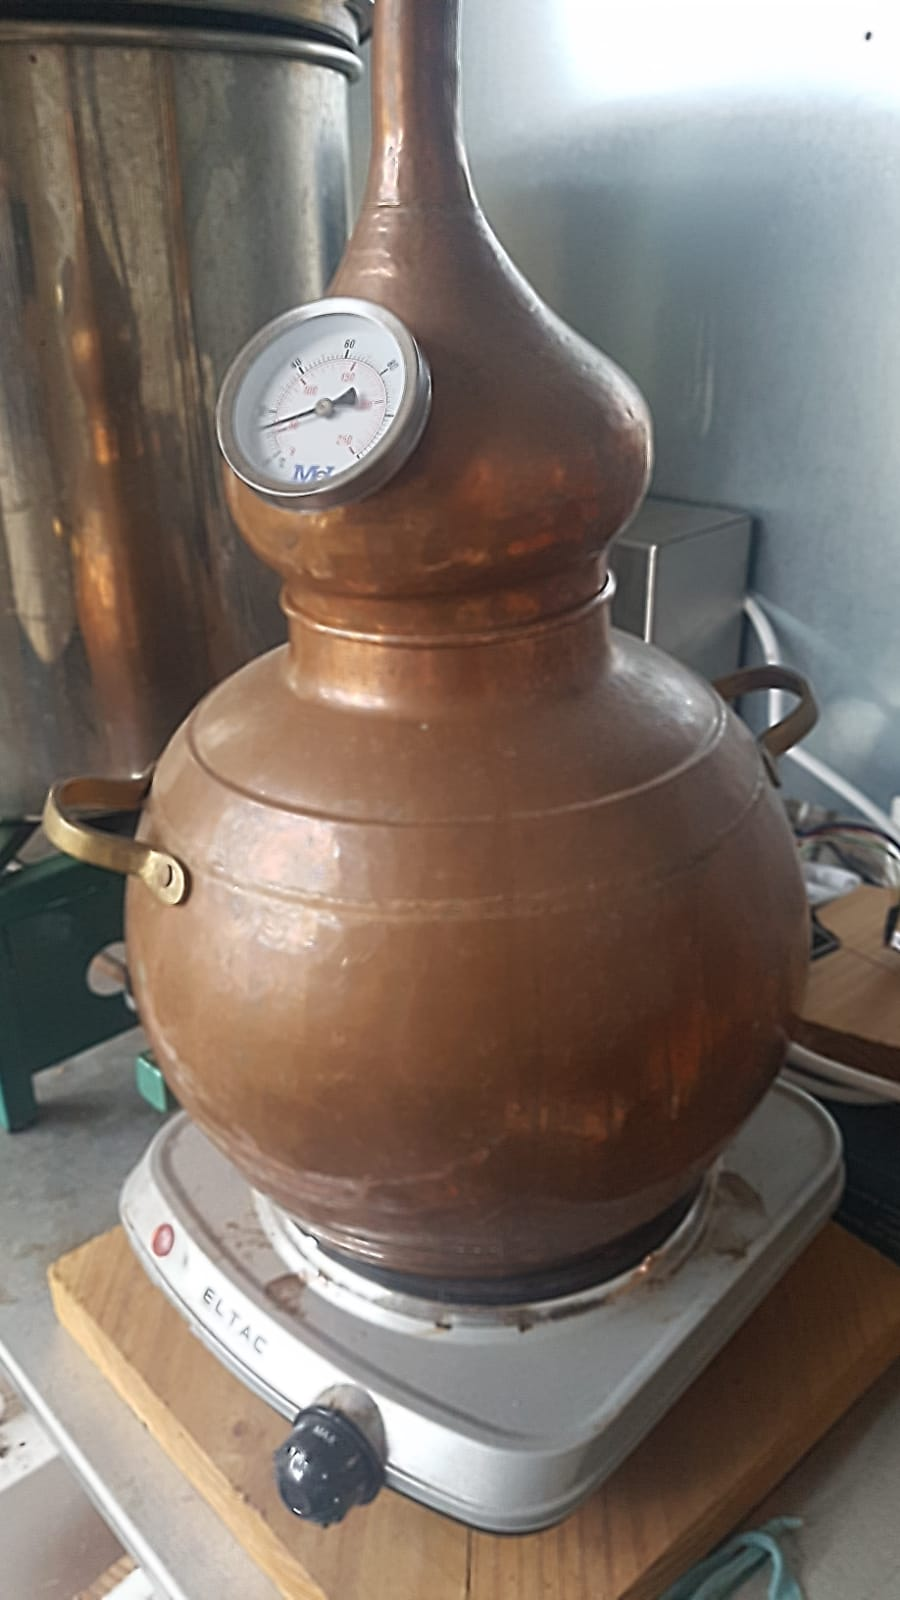
\includegraphics[height=.7\textheight]{images/decorative-still.jpeg}
\end{figure}
\end{frame}

\begin{frame}
\frametitle{Extract the essential component}
Monitor your still:
\begin{figure}
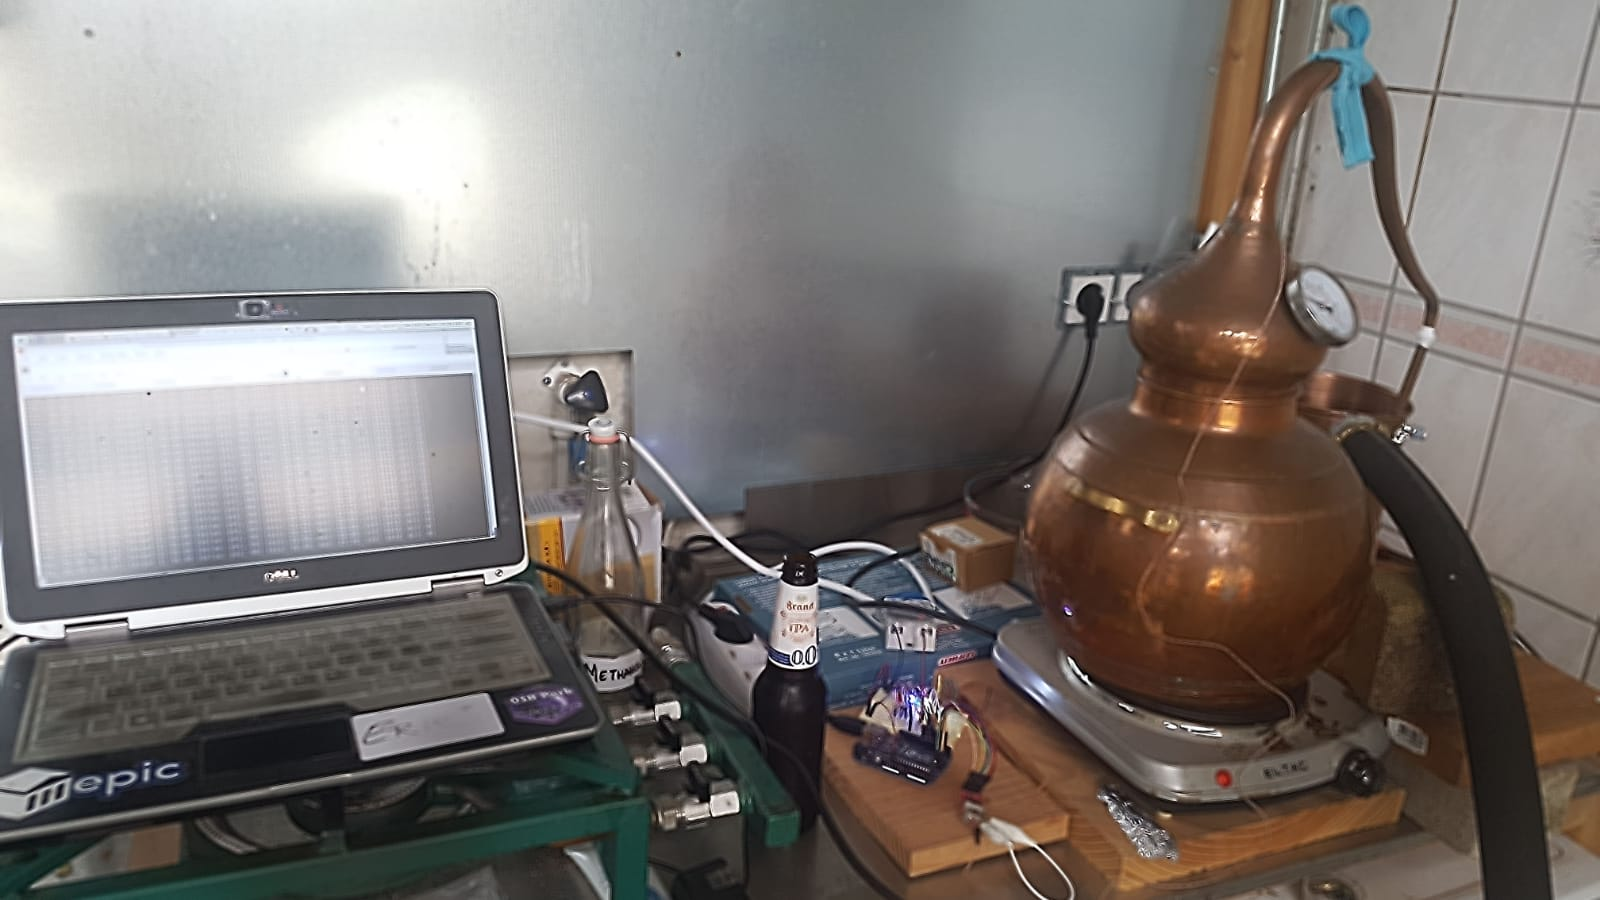
\includegraphics[width=\textwidth]{images/still-wizardry.jpeg}
\end{figure}
Maybe this setup is overkill ....
\end{frame}

\begin{frame}
\frametitle{Safety Tip!}
\begin{figure}
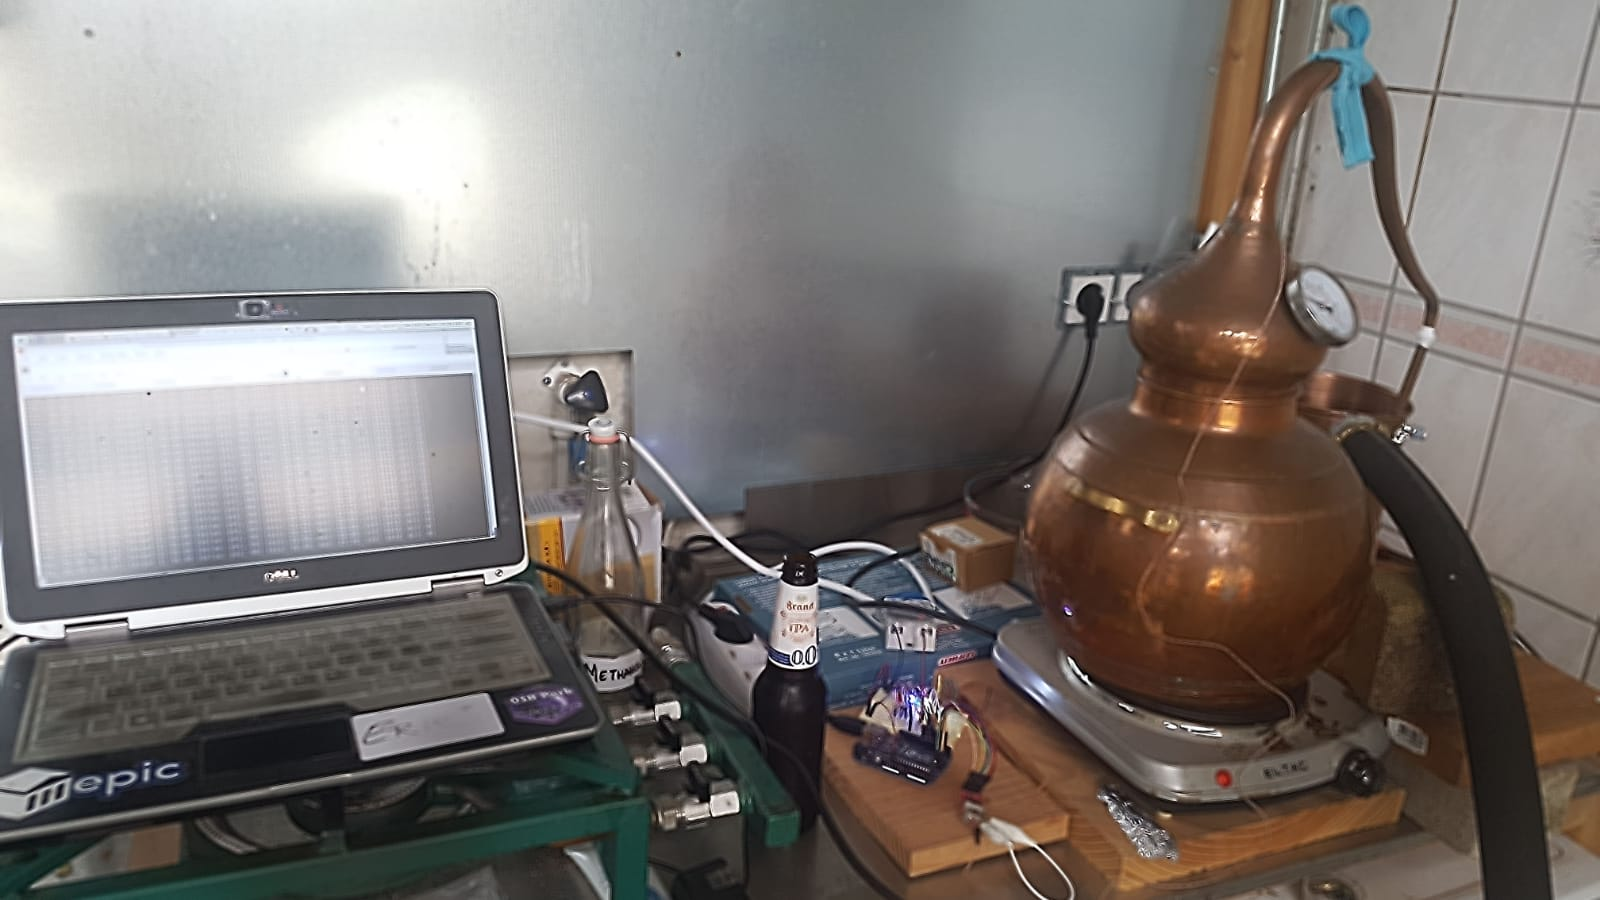
\includegraphics[width=\textwidth]{images/still-wizardry.jpeg}
\end{figure}
\huge{DO NOT TURN ON BURNER UNDER LAPTOP}
\end{frame}


\begin{frame}
\frametitle{Now you have hand sanitizer!}
\begin{figure}
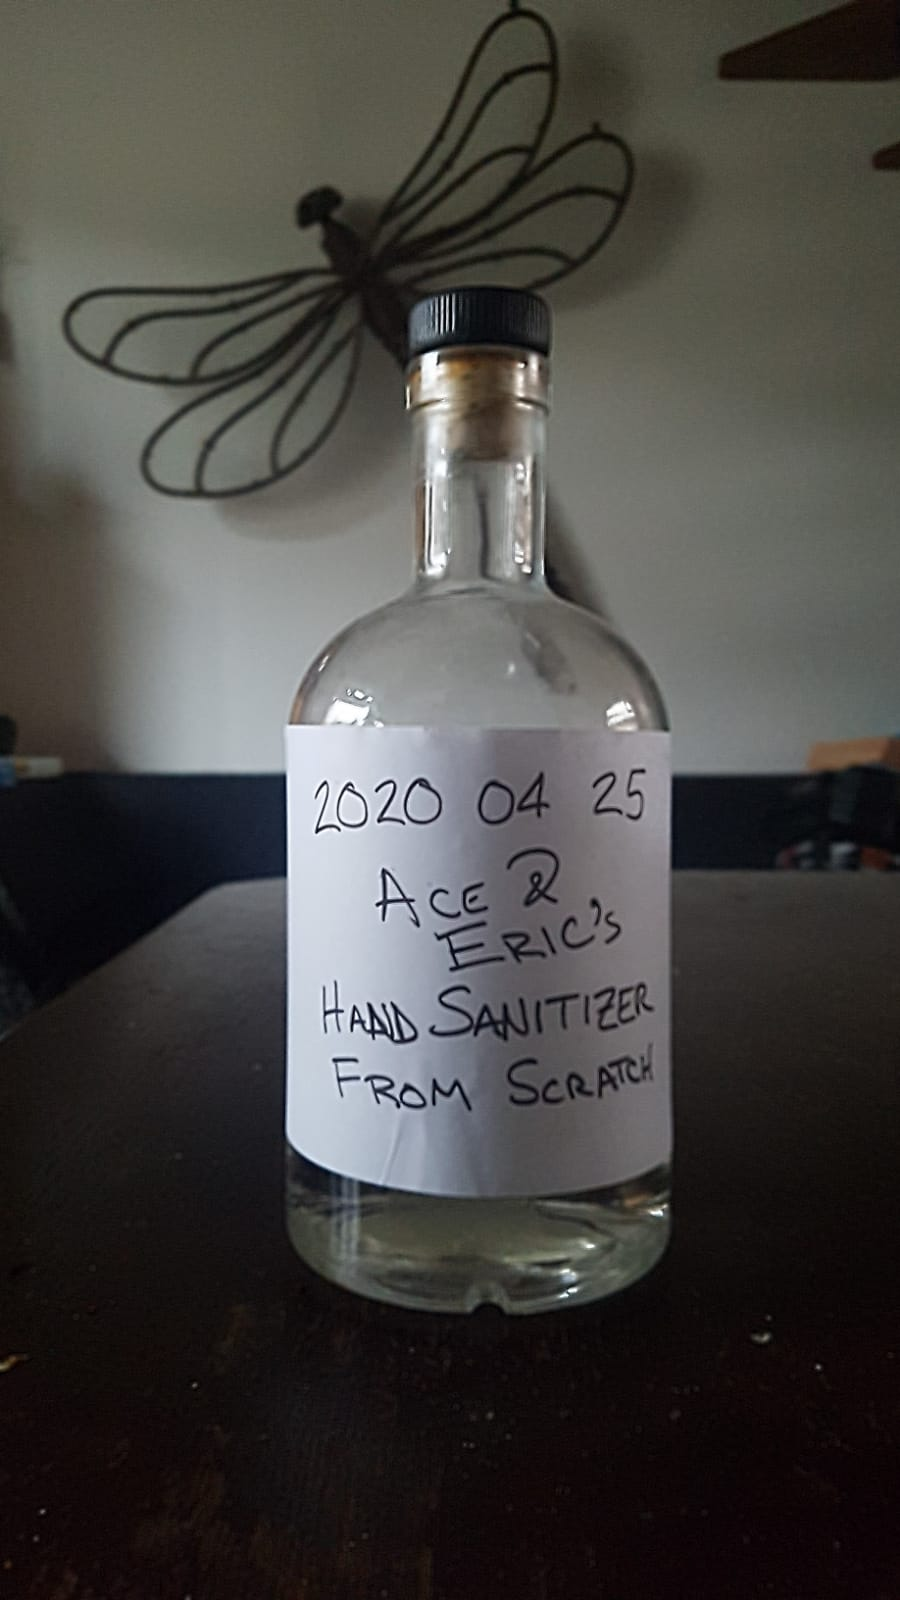
\includegraphics[height=.7\textheight]{images/sanitizer.jpeg}
\end{figure}
\end{frame}

\begin{frame}
\frametitle{But could it be better?}
\huge{Add a charcoal filter?}
\end{frame}

\begin{frame}
\frametitle{Get your old oak branch}
The one that's been drying for a year:
\begin{figure}
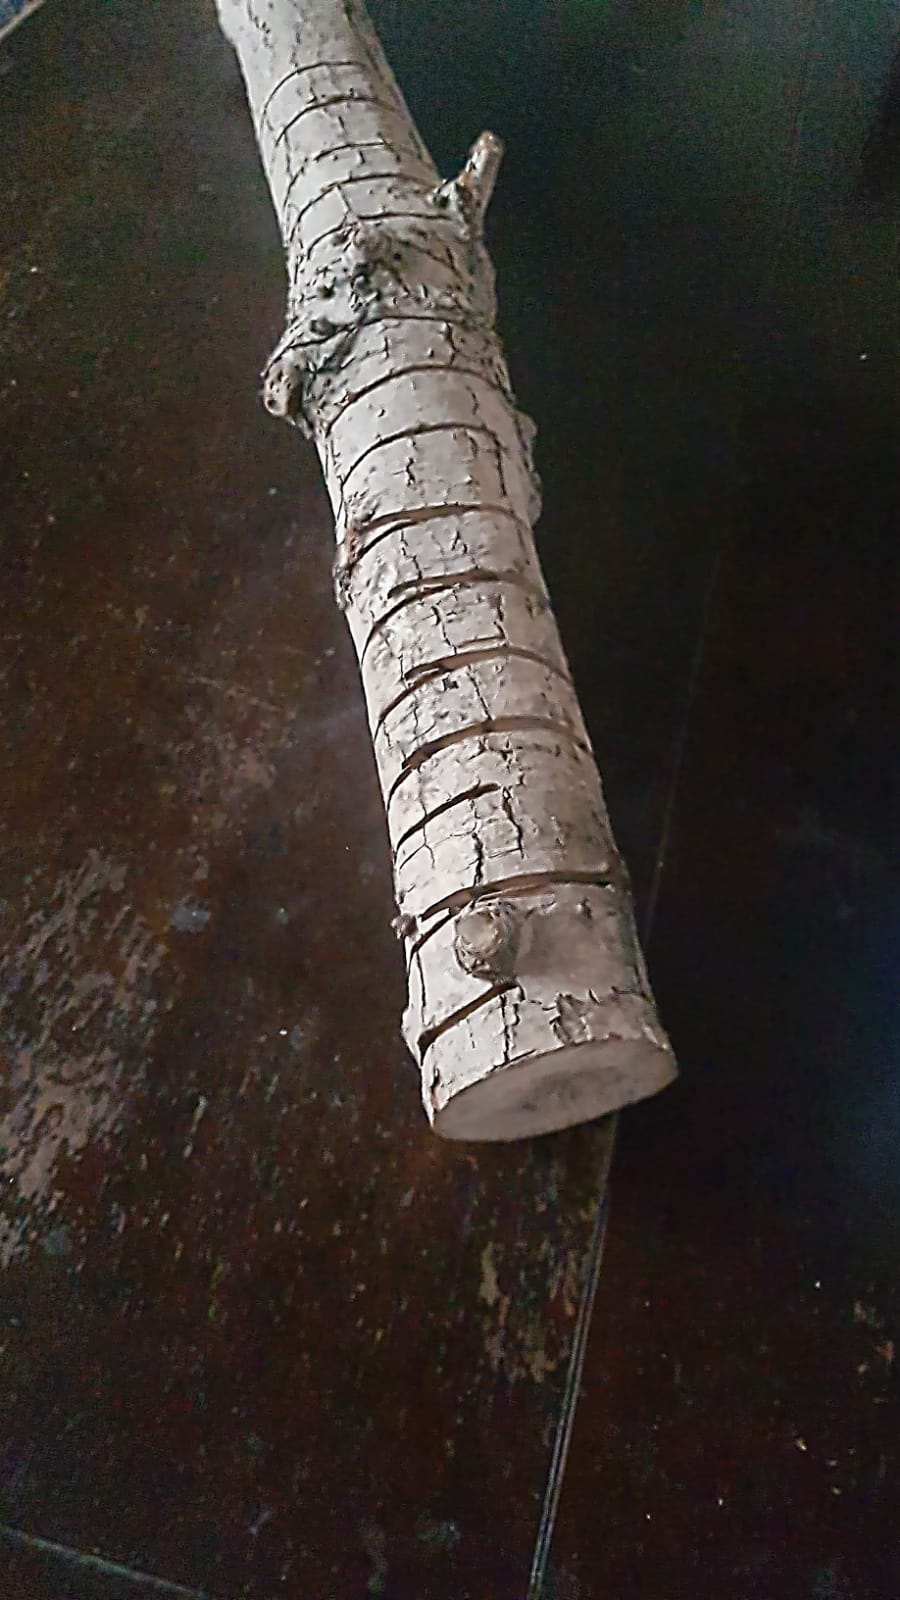
\includegraphics[height=.6\textheight]{images/oak-branch.jpeg}
\end{figure}
Thanks Winold! :-)
\end{frame}

\begin{frame}
\frametitle{Cut in to disks}
\begin{figure}
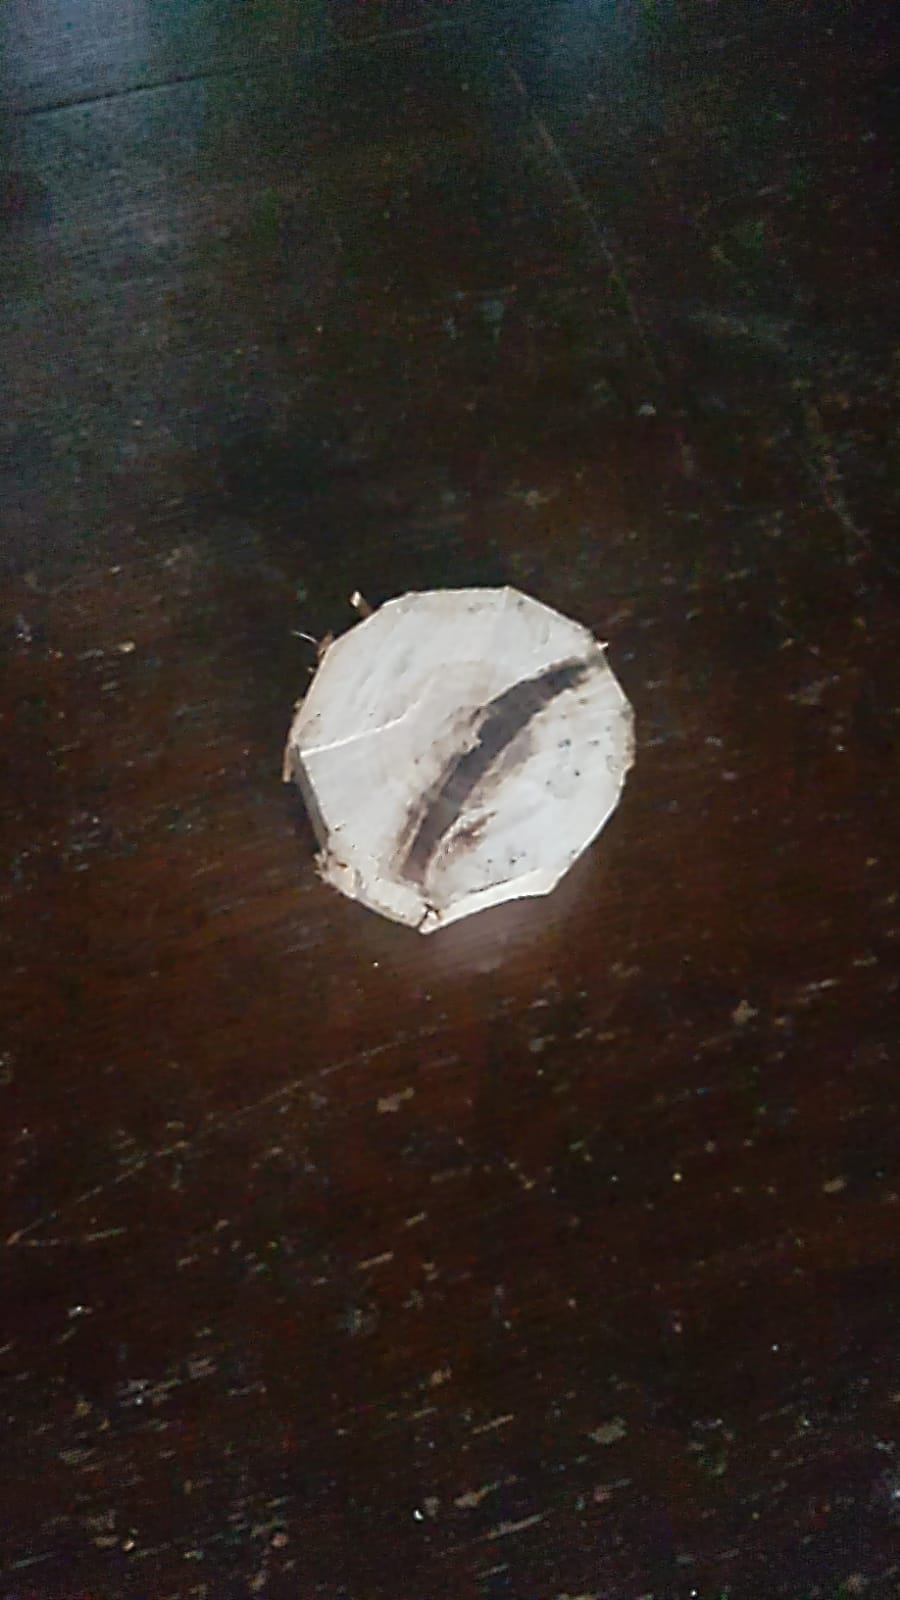
\includegraphics[height=.7\textheight]{images/wooden-disk.jpeg}
\end{figure}
\end{frame}

\begin{frame}
\frametitle{Grill disk}
\begin{figure}
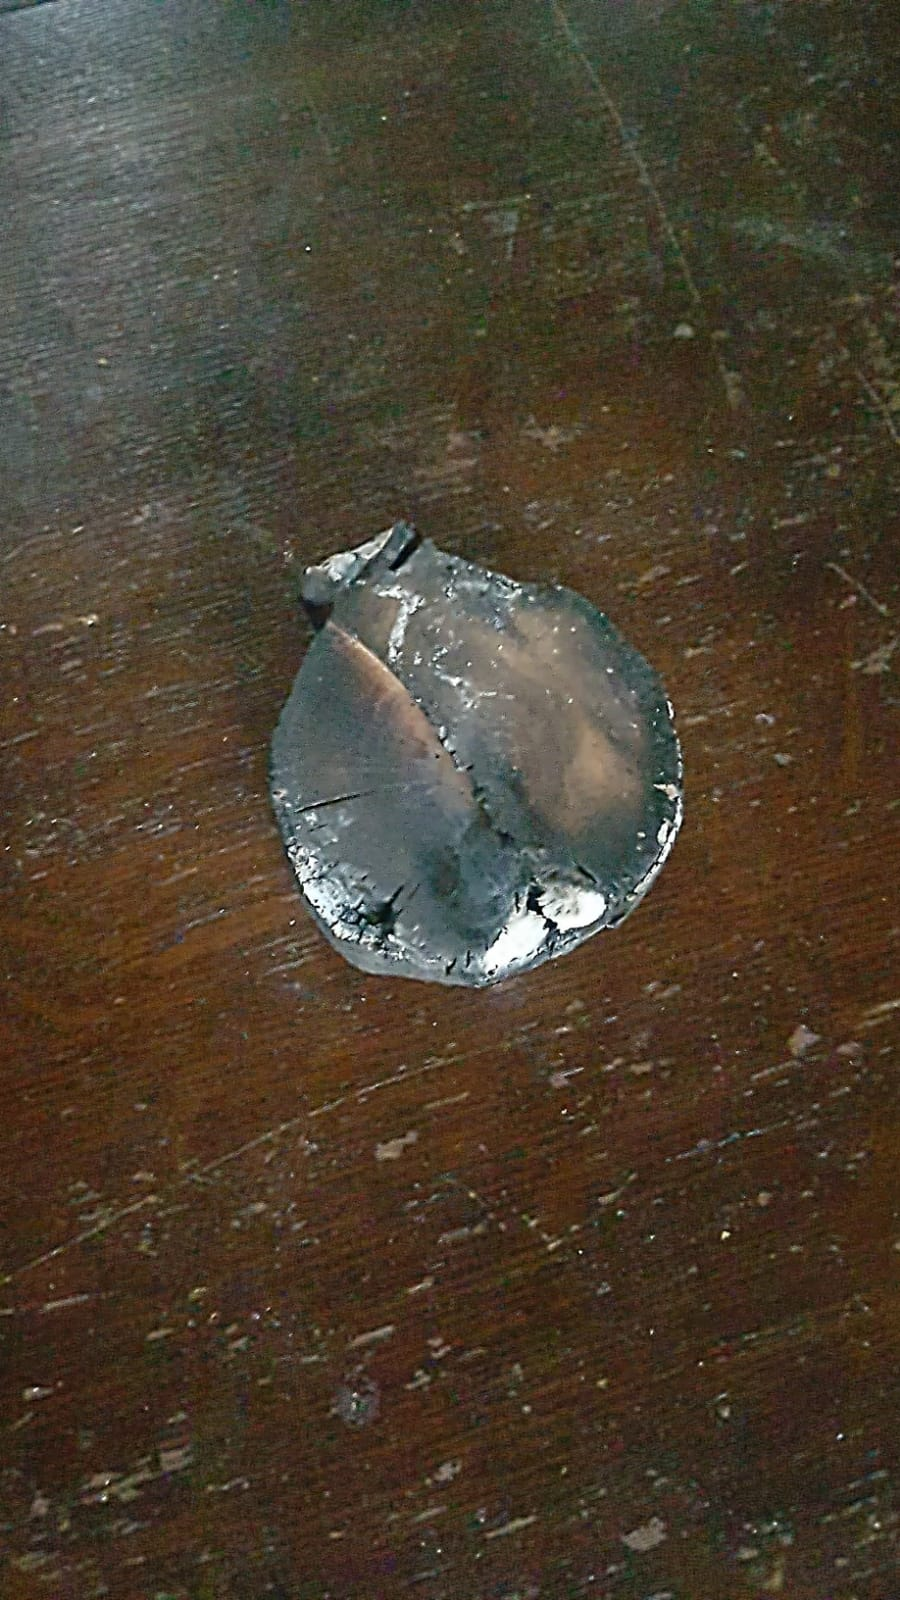
\includegraphics[height=.7\textheight]{images/bbq-disk.jpeg}
\end{figure}
\end{frame}

\begin{frame}
\frametitle{Ordinary jar}
\begin{figure}
\includegraphics[height=.7\textheight]{images/ordinary-jar.jpeg}
\end{figure}
\end{frame}

\begin{frame}
\frametitle{Charcoal filter}
\begin{figure}
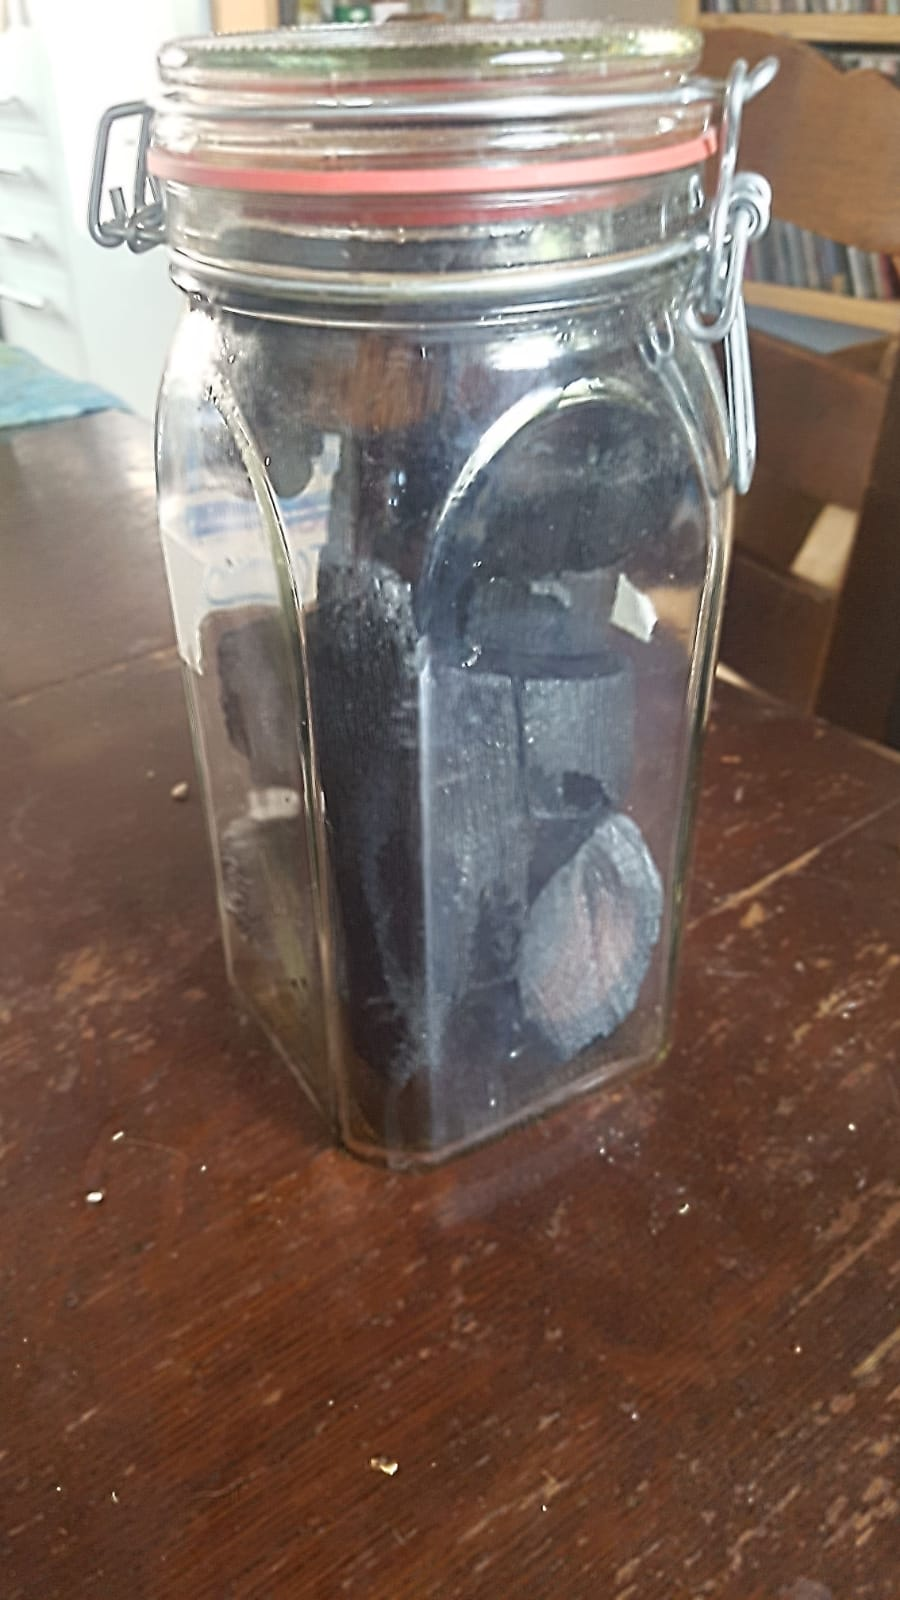
\includegraphics[height=.7\textheight]{images/charcoal-filter.jpeg}
\end{figure}
\end{frame}

\begin{frame}
\frametitle{The color really changes!}
\begin{figure}
\includegraphics[height=.7\textheight]{images/aging-sanitzer.jpeg}
\end{figure}
\end{frame}

\begin{frame}
\frametitle{Now we have improved sanitizer}
\begin{figure}
\includegraphics[height=.7\textheight]{images/aged-sanitizer.jpeg}
\end{figure}
\end{frame}


\begin{frame}
\frametitle{Redundancy and Scale-out}
Be sure to make enough for each of your individual visitors to keep
their hands clean.
\begin{figure}
\includegraphics[height=.7\textheight]{images/scale-out.jpeg}
\end{figure}
\end{frame}

\begin{frame}
\frametitle{Thank you}
\huge{Stay Safe and keep those hands sanitized!}\newline
\begin{itemize}
\item eric.herman@gmail.com
\item github.com/ericherman
\item twitter.com/Eric\_Herman
\end{itemize}
\end{frame}

\end{document}
